\documentclass{article}

\title{P6 Report}
\author{Nick Werle}

\usepackage{hyperref}
\usepackage{graphicx}

\begin{document}
\maketitle
\section{Preamble}
All necessary files will be uploaded to my githb repository at \url{https://github.com/NickWer/CEG3900_P6b}

\section{Task 1}
Deliverables: See figure 2
I created four ubuntu server instances on AWS EC2 and then manually segmented each file into 13 rows (52 hashes to begin).
I let the four instances of John run for ~3 hours and managed, as expected to crack the guest password (guest007).

For the APK, I created a relatively simple setup: A button, a status label, and four scrollbox'd \texttt{TextView}s for the standard output of each computer. When the button is click, I spin up for AsynTasks that use \texttt{Process.getRuntime().exe()} to run an ssh command. One hurdle that I had to overcome was that android restricts reading assets to strictly from the APK. I found on stack overflow a small bit of code that I modified to suit my neads - it reads the file from the assets folder and copies it into an unarchived file in the temp folder, where it can then be referenced by the ssh command. 

I believe this solution will only work on rooted devices. Running it without causes the following error:
\begin{verbatim}
W/System.err: java.io.IOException: Cannot run program "ssh": error=13, Permission denied
W/System.err:     at java.lang.ProcessBuilder.start(ProcessBuilder.java:983)
W/System.err:     at java.lang.Runtime.exec(Runtime.java:691)
W/System.err:     at java.lang.Runtime.exec(Runtime.java:524)
W/System.err:     at java.lang.Runtime.exec(Runtime.java:421)
W/System.err:     at com.example.nick.jtrrunner.MainActivity$runSsh.doInBackground(MainActivity.java:74)
W/System.err:     at com.example.nick.jtrrunner.MainActivity$runSsh.doInBackground(MainActivity.java:29)
W/System.err:     at android.os.AsyncTask$2.call(AsyncTask.java:304)
W/System.err:     at java.util.concurrent.FutureTask.run(FutureTask.java:237)
W/System.err:     at android.os.AsyncTask$SerialExecutor$1.run(AsyncTask.java:243)
W/System.err:     at java.util.concurrent.ThreadPoolExecutor.runWorker(ThreadPoolExecutor.java:1133)
W/System.err:     at java.util.concurrent.ThreadPoolExecutor$Worker.run(ThreadPoolExecutor.java:607)
W/System.err:     at java.lang.Thread.run(Thread.java:761)
W/System.err: Caused by: java.io.IOException: error=13, Permission denied
W/System.err:     at java.lang.UNIXProcess.forkAndExec(Native Method)
\end{verbatim}

Figure 2 shows the main screen of my APK - however without root I cannot get much futher. To display progress to the user, I keep the stdio output in a string, and whenever more comes in, it uses the publishProgress method to update the UI from the UI thread, which I do know works.

	\begin{figure}[ht]
        \centerline{
            \includegraphics[width=7.5in]{img/t1s1.png}
        }
		\centering
		\caption{Task 1 - Four instances running at once over ssh}
	\end{figure}
	\begin{figure}[ht]
        \centerline{
            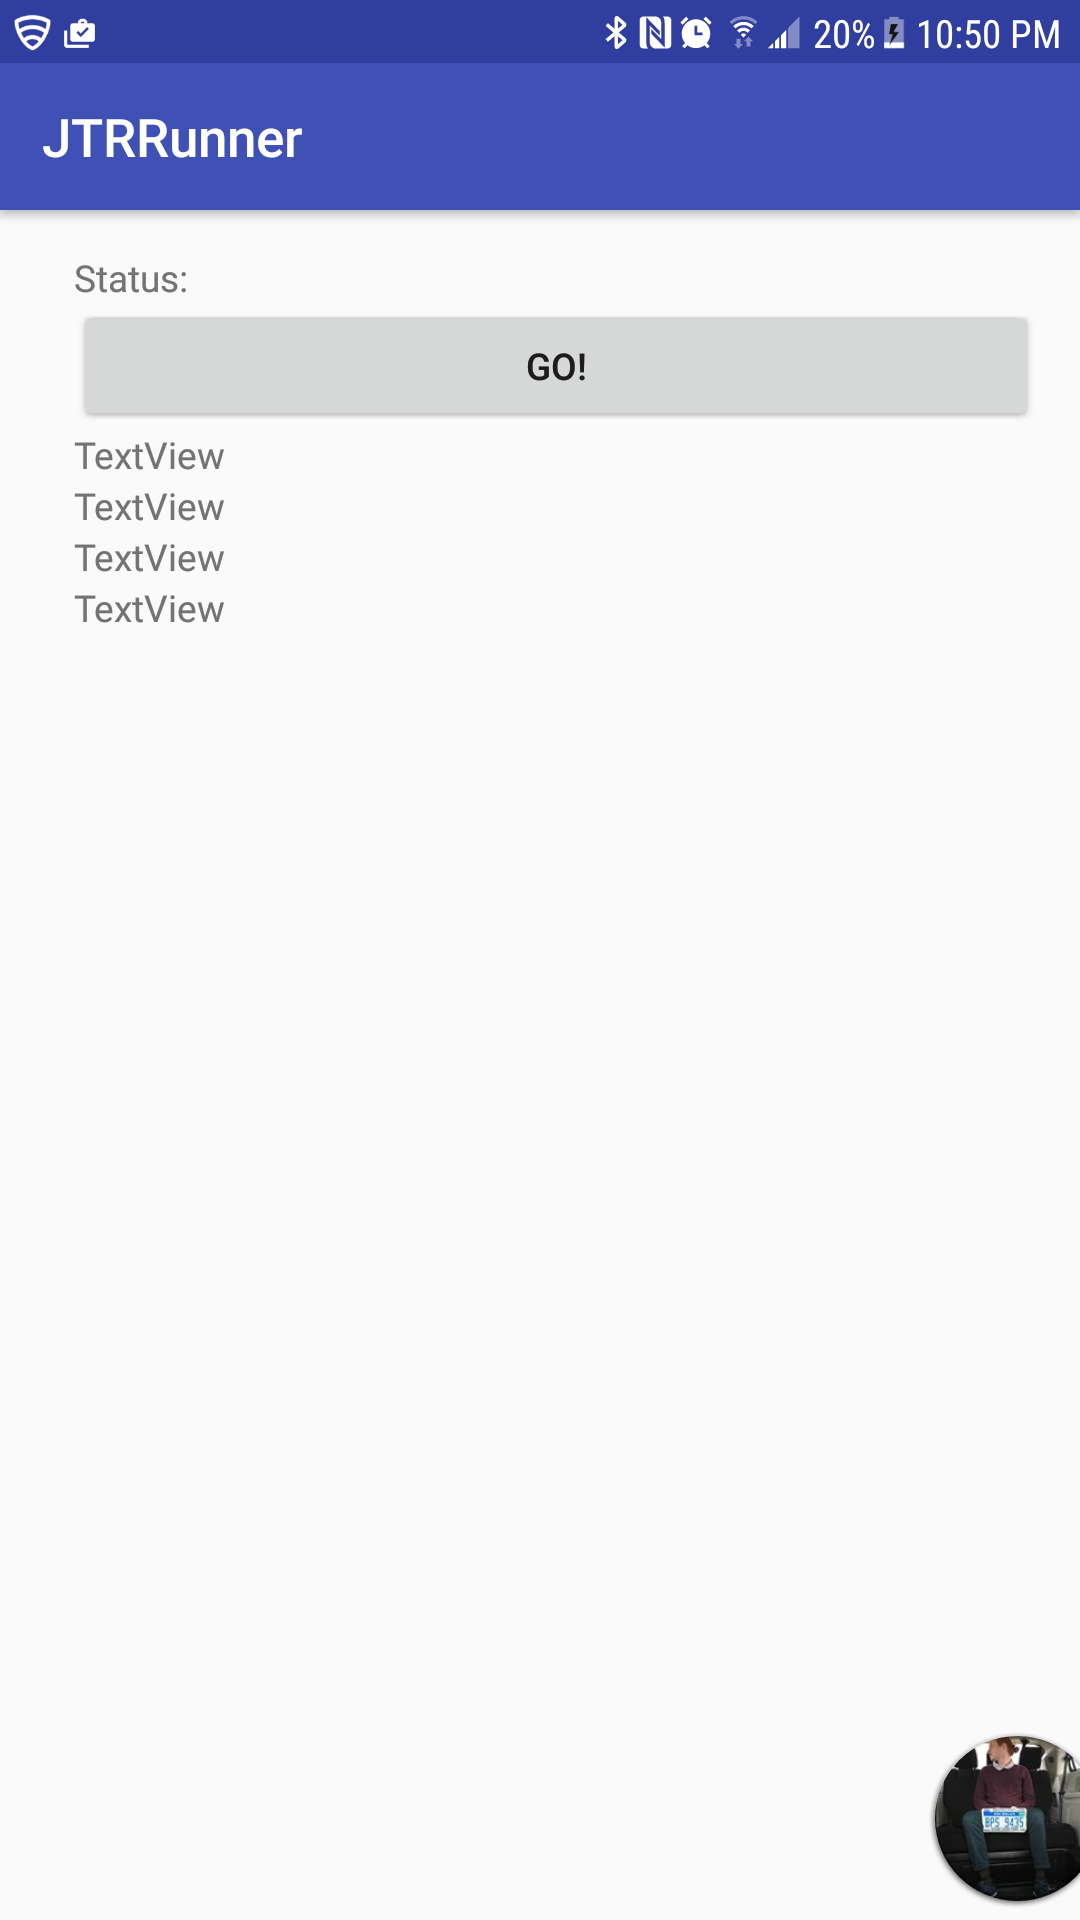
\includegraphics[width=3in]{img/t1s2.png}
        }
		\centering
		\caption{Task 1 - APK Running, insofar as it is able without root.}
	\end{figure}


\clearpage

\section{Task 2}
I was able to run hashcat on my desktop at home, which natively runs Ubuntu 16.04 (as opposed to my laptop that I `dist-uprade`ed to 16.04), and also includes an NVidia GPU as opposed to my laptop's AMD card.
I attempted to make a docker to see if it would run correctly inside of there, but it suffered from the same drivers issue that I struggled with before, and it didn't seem worth it to install those in the docker, too.
Anyways, I ran the hashcat program twice. Once with attack mode 0:

\begin{verbatim}
eb61eead90e3b899c6bcbe27ac581660:HELLO
2ac9cb7dc02b3c0083eb70898e549b63:Password1
75b71aa6842e450f12aca00fdf54c51d:P455w0rd
2c9341ca4cf3d87b9e4eb905d6a3ec45:Test1234
958152288f2d2303ae045cffc43a02cd:MYSECRET
eb61eead90e3b899c6bcbe27ac581660:HELLO
2ac9cb7dc02b3c0083eb70898e549b63:Password1
75b71aa6842e450f12aca00fdf54c51d:P455w0rd
2c9341ca4cf3d87b9e4eb905d6a3ec45:Test1234
958152288f2d2303ae045cffc43a02cd:MYSECRET
\end{verbatim}

Attack mode 3 (bruteforcing) was insanely slow, and I suspect would not have been able to find all of the passwords anyways, at least not today.
\begin{verbatim}
eb61eead90e3b899c6bcbe27ac581660:HELLO
2ac9cb7dc02b3c0083eb70898e549b63:Password1
75b71aa6842e450f12aca00fdf54c51d:P455w0rd
2c9341ca4cf3d87b9e4eb905d6a3ec45:Test1234
958152288f2d2303ae045cffc43a02cd:MYSECRET
\end{verbatim}

\textbf{Rules File} I annotated the combinator rule file:
\begin{verbatim}
## rule: case recovery
## limits: capitalized rules only char positions 3 to 7
## example: annalove ---> AnnaLove
## extras: none
#noop
:
#all lowercase
l
#capitalize first letter
c
#uppercase all letters
u

#capitalize first letter, toggle case at position N (3..7)
c T3
c T4
c T5
c T6
c T7

## rule: experienced effective
## limits: none
## example: FringeDevision ---> fringedevision2009
## extras: lower case only

#Lowercase all letters, append  1, 2, 123, 2007, 2008, 2009
l $1
l $2
l $1$2$3
l $2$0$0$7
l $2$0$0$8
l $2$0$0$9

## rule: hyphen variety
## limits: insert at char positions 3 to 7
## example: theobserver ---> the observer
## extras: lower case only

#lowercase all letters, add space/&/-/. at position N
l i3 
l i4 
l i5 
l i6 
l i7 
l i3&
l i4&
l i5&
l i6&
l i7&
l i3+
l i4+
l i5+
l i6+
l i7+
l i3-
l i4-
l i5-
l i6-
l i7-
l i3.
l i4.
l i5.
l i6.
l i7.

\end{verbatim}

\textbf{Android APK}
My android APK for this problem was extremely similar to the previous. All I did was:
\begin{enumerate}
\item only run one instance
\item Added inputs for hashes and wordlist
\item pointed it at my home computer
\item created a user and used the server ssh key from before. Most certainly NOT going to commit my actual private key to a public repo.
\item This time I use the shell interactively rather than doing a remote execution. I download the hashes and wordlist files using curl.
\item Finally I run hashcat and provide output as before.
\end{enumerate}
An unfortunate side effect is that it suffers from the same permissions error. I am not sure how to get past this.

	\begin{figure}[ht]
        \centerline{
            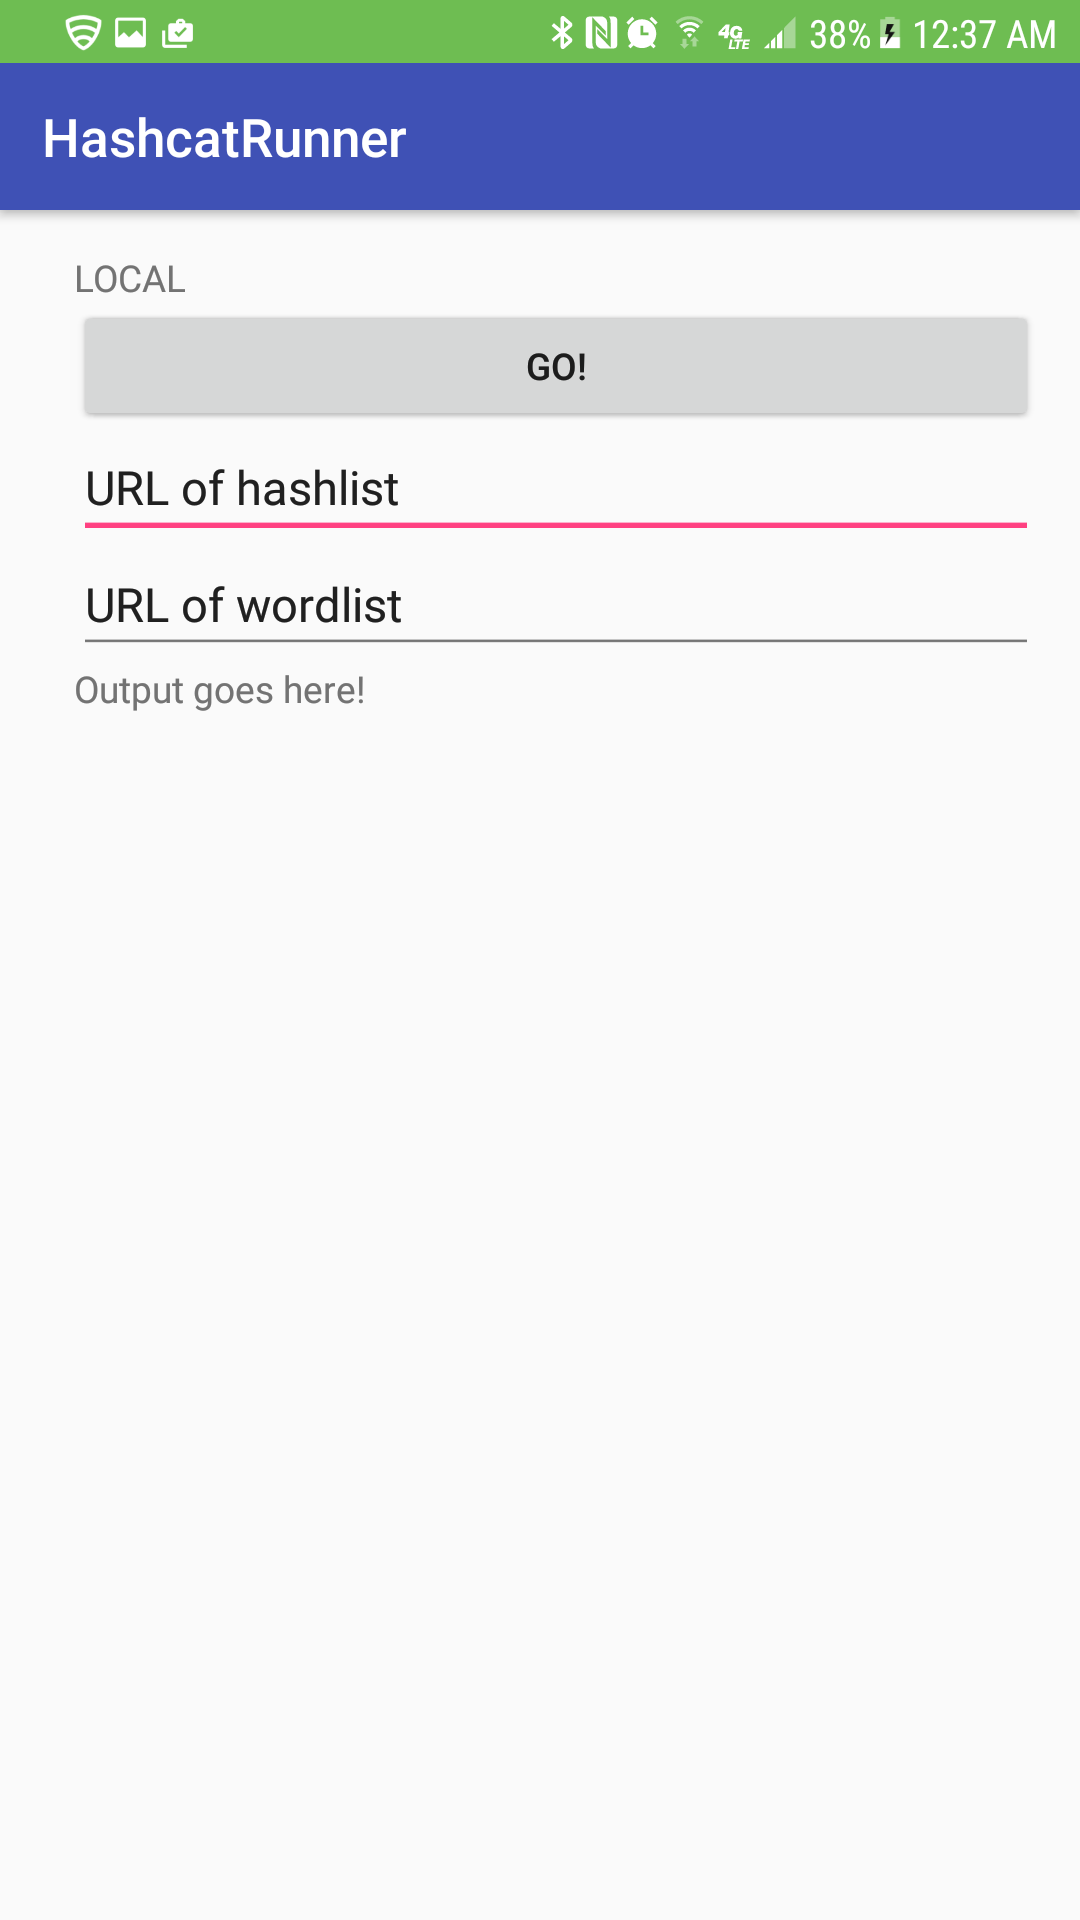
\includegraphics[width=3in]{img/t2s1.png}
        }
		\centering
		\caption{Task 2 - APK Running, insofar as it is able without root.}
	\end{figure}
	\clearpage


\section{Task 3}
During my previous sumission I created the docker container for Task 2. I was able to trivially transfer my hashcat setup to the new machine.
To test it, I modified my dockerfile slightly from before:


\begin{verbatim}
FROM hihouhou/hashcat

ADD http://cecs.wright.edu/~pmateti/Courses/3900/Lectures/Assignments/hashes-md5.txt /root/
ADD http://downloads.skullsecurity.org/passwords/rockyou.txt.bz2

RUN apt-get install -y bzip2
RUN cd /root/ && bzip2 -d rockyou.txt.bz2
\end{verbatim}

and then the output:
\begin{verbatim}
[s]tatus [p]ause [r]esume [b]ypass [q]uit =>

Input.Mode: Dict (/root/rockyou.txt)
Index.....: 5/5 (segment), 553093 (words), 5720127 (bytes)
Recovered.: 5/8 hashes, 0/1 salts
Speed/sec.: 4.38M plains, 4.38M words
Progress..: 553093/553093 (100.00%)
Running...: 00:00:00:01
Estimated.: --:--:--:--


Started: Fri Apr  7 04:09:48 2017
Stopped: Fri Apr  7 04:09:53 2017
ubuntu@ip-172-31-26-17:~$
\end{verbatim}

The hashes cracked:
\begin{verbatim}
2ac9cb7dc02b3c0083eb70898e549b63:Password1
eb61eead90e3b899c6bcbe27ac581660:HELLO
75b71aa6842e450f12aca00fdf54c51d:P455w0rd
2c9341ca4cf3d87b9e4eb905d6a3ec45:Test1234
958152288f2d2303ae045cffc43a02cd:MYSECRET
\end{verbatim}

Previously, I found this article \url{http://blog.trifork.com/2013/12/24/docker-from-a-distance-the-remote-api/}. It appeared that if I used that, I could trivially implement these android applications by just having the buttons send AJAX.

That said, it ended up actually being way easier to just throw hashcat and it's dependencies into the main folder and run it. Sadly, tonight will not be the night for cool experiments.

This apk was a trivial modification of the previous: all I did was modify the previous one to point at the new remote address (i.e.\ the EC2 instance rather than my home PC).

	\begin{figure}[ht]
        \centerline{
            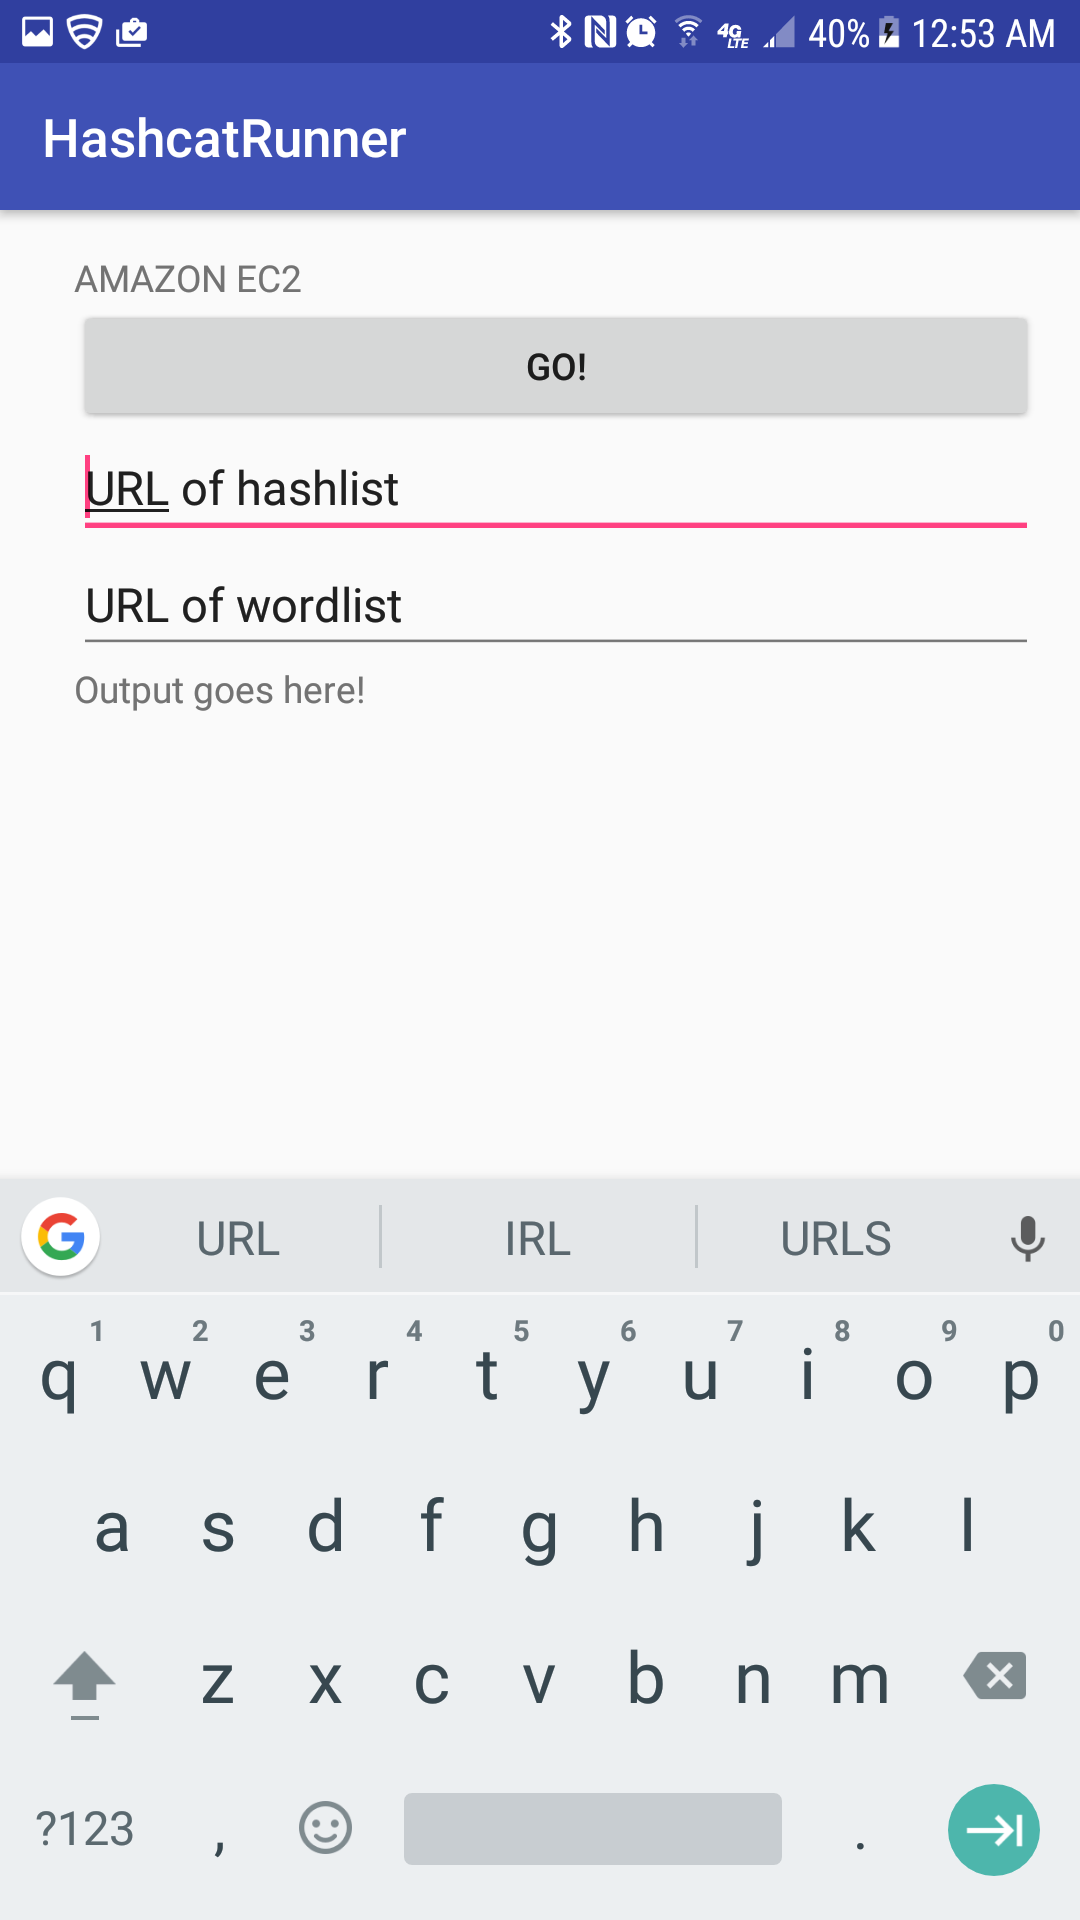
\includegraphics[width=3in]{img/t3s1.png}
        }
		\centering
		\caption{Task 3 - APK Running, insofar as it is able without root.}
	\end{figure}
	\clearpage


\section{Task 4}
I feel like I am very close - I am just really struggling to get cassandra to start from inside the docker, and not having much luck with linking an outside docker to this one.

Here is the post I made in pilot:
\hrule

Trying to construct a docker image for painbow. Should I run a second docker for cassandra and link it to the painbow instance as they do in the docs at \url{https://hub.docker.com/_/cassandra/}?

Or should I run cassandra inside of my painbow docker - which is what I'm currently trying to do after giving up on the previous?

I get the following error:

\begin{verbatim}
nick@nick-lenovo ~/D/C/P/Task4> docker run -i nick/task4 bin/painbow --migrate
SLF4J: Failed to load class "org.slf4j.impl.StaticLoggerBinder".
SLF4J: Defaulting to no-operation (NOP) logger implementation
SLF4J: See http://www.slf4j.org/codes.html#StaticLoggerBinder for further details.
Exception in thread "main" com.datastax.driver.core.exceptions.NoHostAvailableException: All host(s) tried for query failed (tried: /127.0.0.1:9042 (com.datastax.driver.core.TransportException: [/127.0.0.1:9042] Cannot connect))
    at com.datastax.driver.core.ControlConnection.reconnectInternal(ControlConnection.java:227)
    at com.datastax.driver.core.ControlConnection.connect(ControlConnection.java:82)
    at com.datastax.driver.core.Cluster$Manager.init(Cluster.java:1307)
    at com.datastax.driver.core.Cluster.init(Cluster.java:159)
    at com.datastax.driver.core.Cluster.connect(Cluster.java:249)
    at us.yellosoft.painbow.Painbow.main(Painbow.java:154)

\end{verbatim}
Basically: I'm unable to start cassandra within my docker.

Running `service cassandra start` outputs an error, too. Based on preliminary research this is expected when inside of a docker (security reasons) and non-fatal, but i'm not conviced.

docker run -i nick/task4 service cassandra start
/etc/init.d/cassandra: 72: ulimit: error setting limit (Operation not permitted)

Taking any and all ideas.

My dockerfile is basically a merge of the gradle and cassandra dockerfiles, plus RUN statements to build painbow.
\hrule

\section{Task 5}
See figures 5-10 for screenshots of apk, and Task 5 folder.

My apk works as expected and provides very nice feedback. I was very impressed with the Nbcxz library - it is fast and clearly effective. Something like this would definitely be wise to build into future applications, provided it can scale well (I mean, people don't set their passwords very often, but it might serve as a DoS vector or something similar...)

Anyways you can tell I thought it was interesting because I took a groundbreaking 5th screenshot.

	\begin{figure}[ht]
        \centerline{
            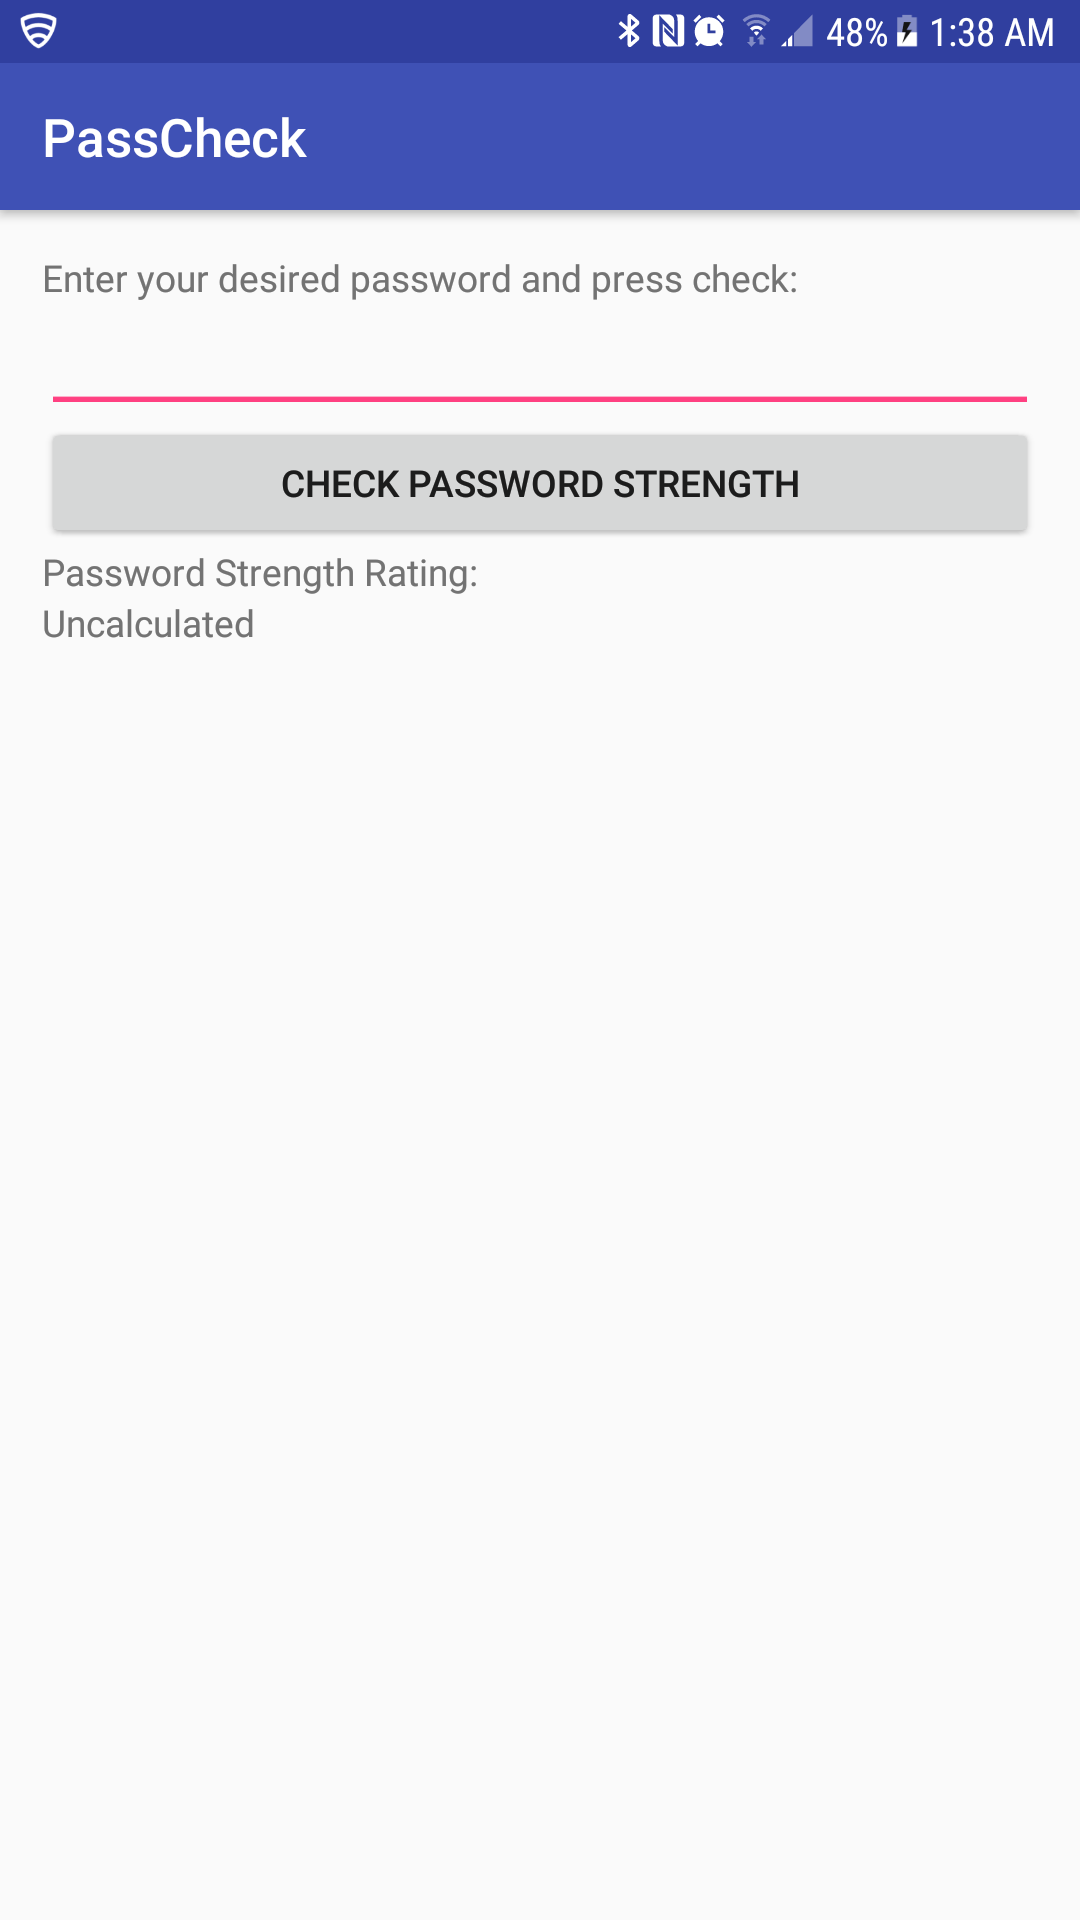
\includegraphics[width=3in]{img/t5s1.png}
        }
		\centering
		\caption{Task 5 - Starting screen}
	\end{figure}

	\begin{figure}[ht]
        \centerline{
            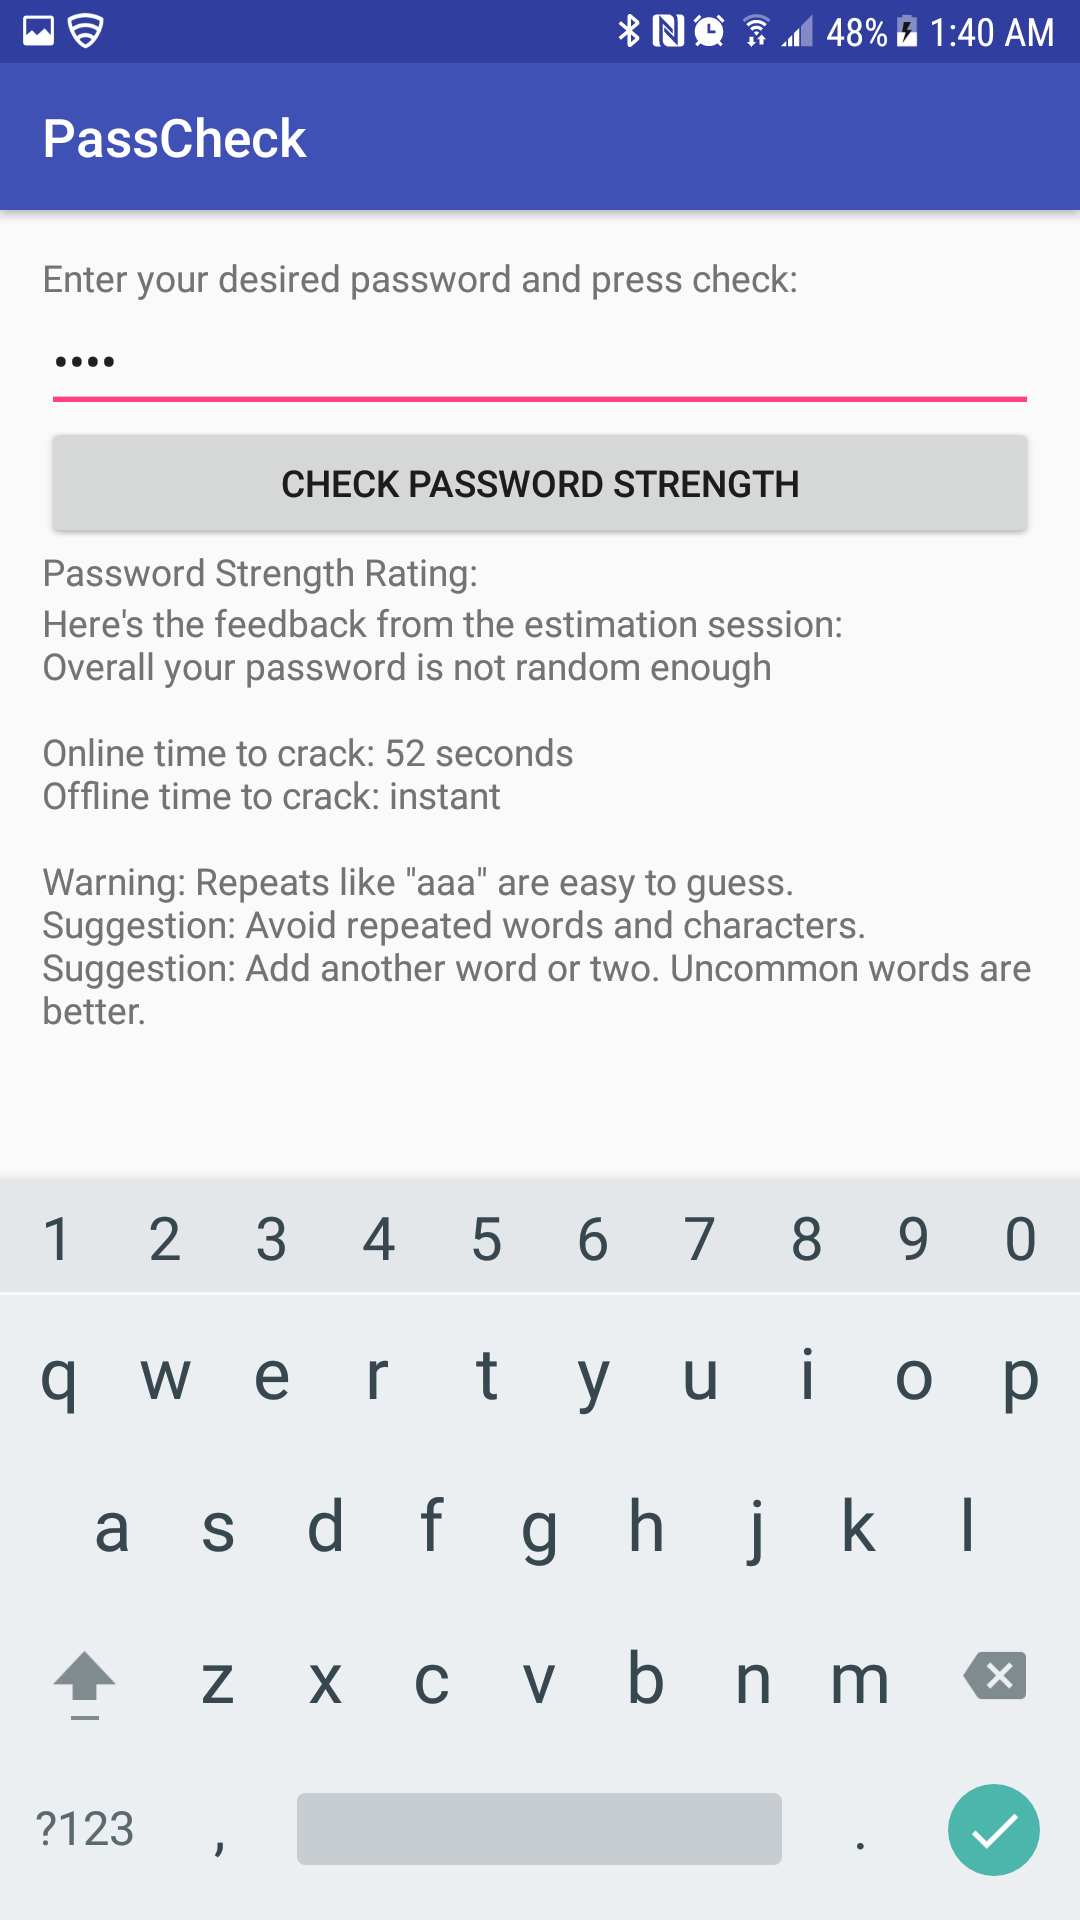
\includegraphics[width=3in]{img/t5s2.png}
        }
		\centering
		\caption{Task 5 - Using a trivial password: aaa}
	\end{figure}

	\begin{figure}[ht]
        \centerline{
            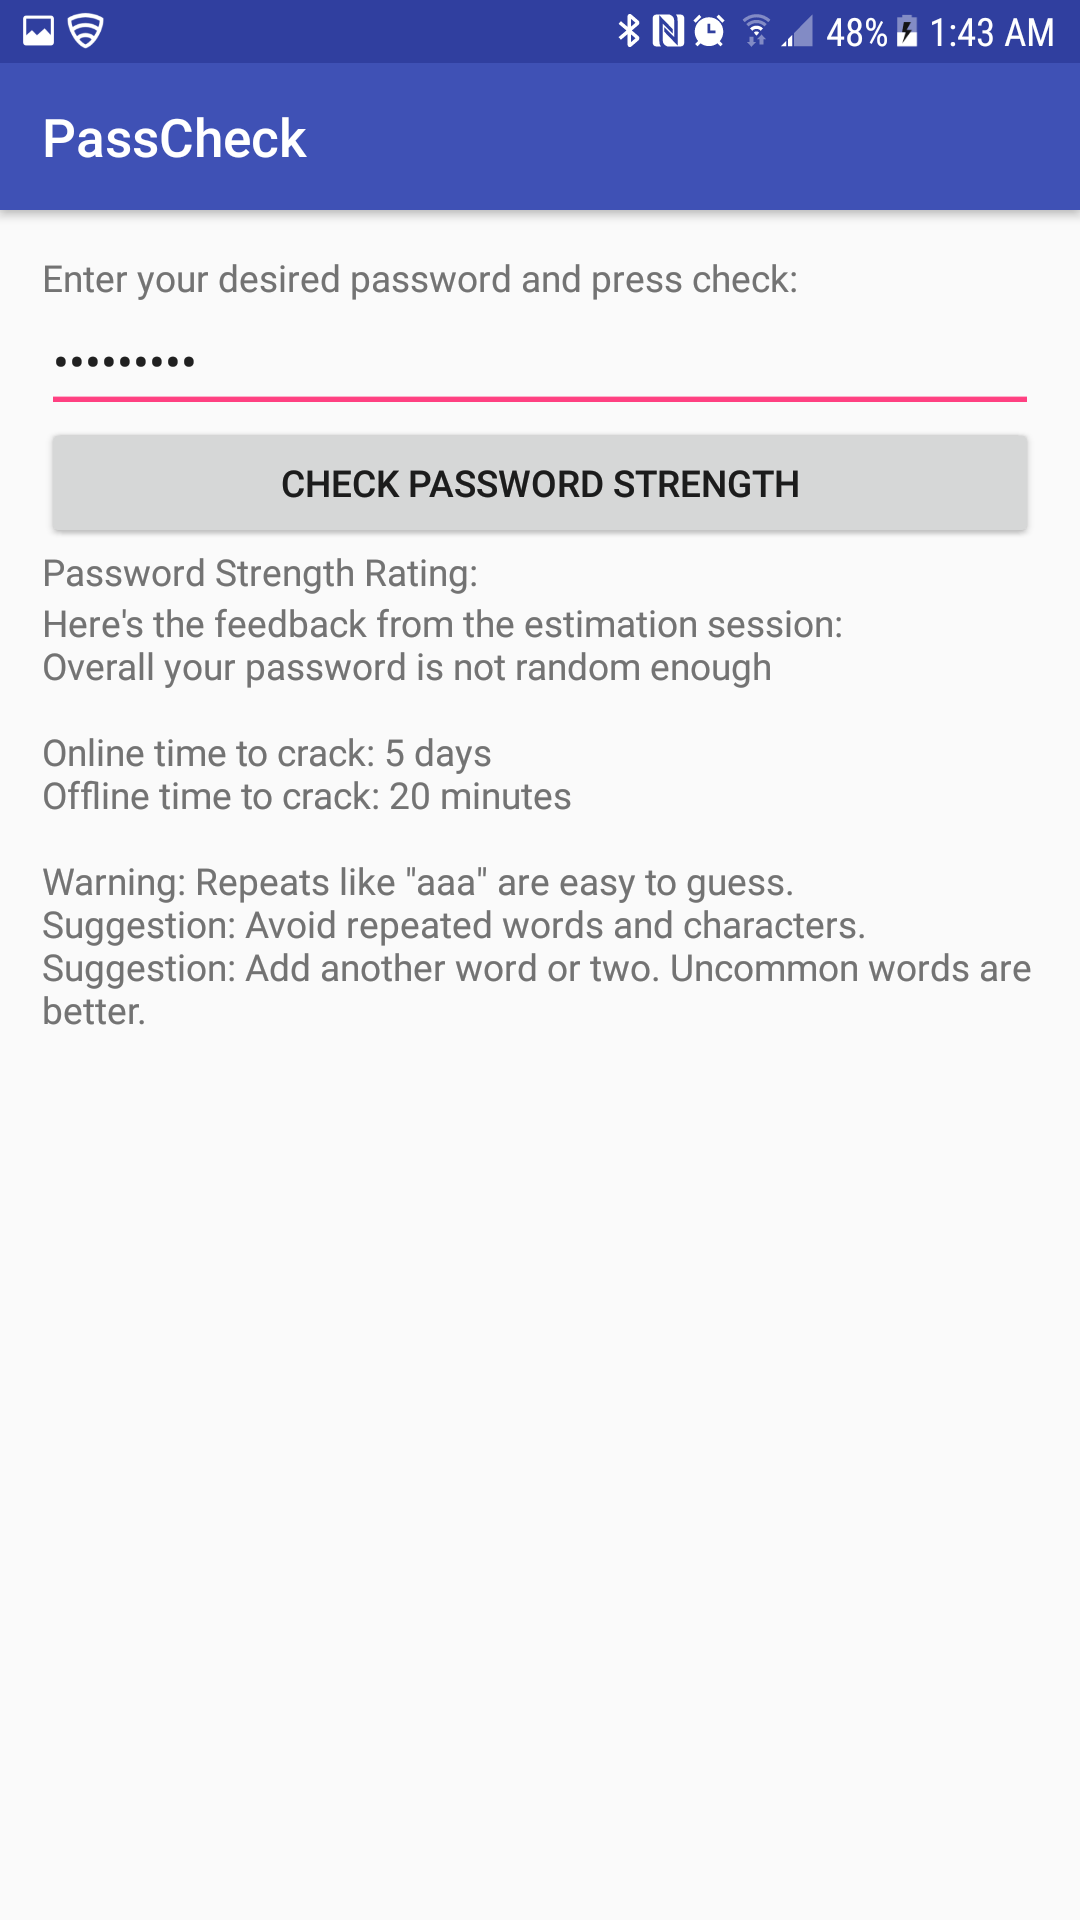
\includegraphics[width=3in]{img/t5s3.png}
        }
		\centering
		\caption{Task 5 - Using a trivial password with random characters}
	\end{figure}

	\begin{figure}[ht]
        \centerline{
            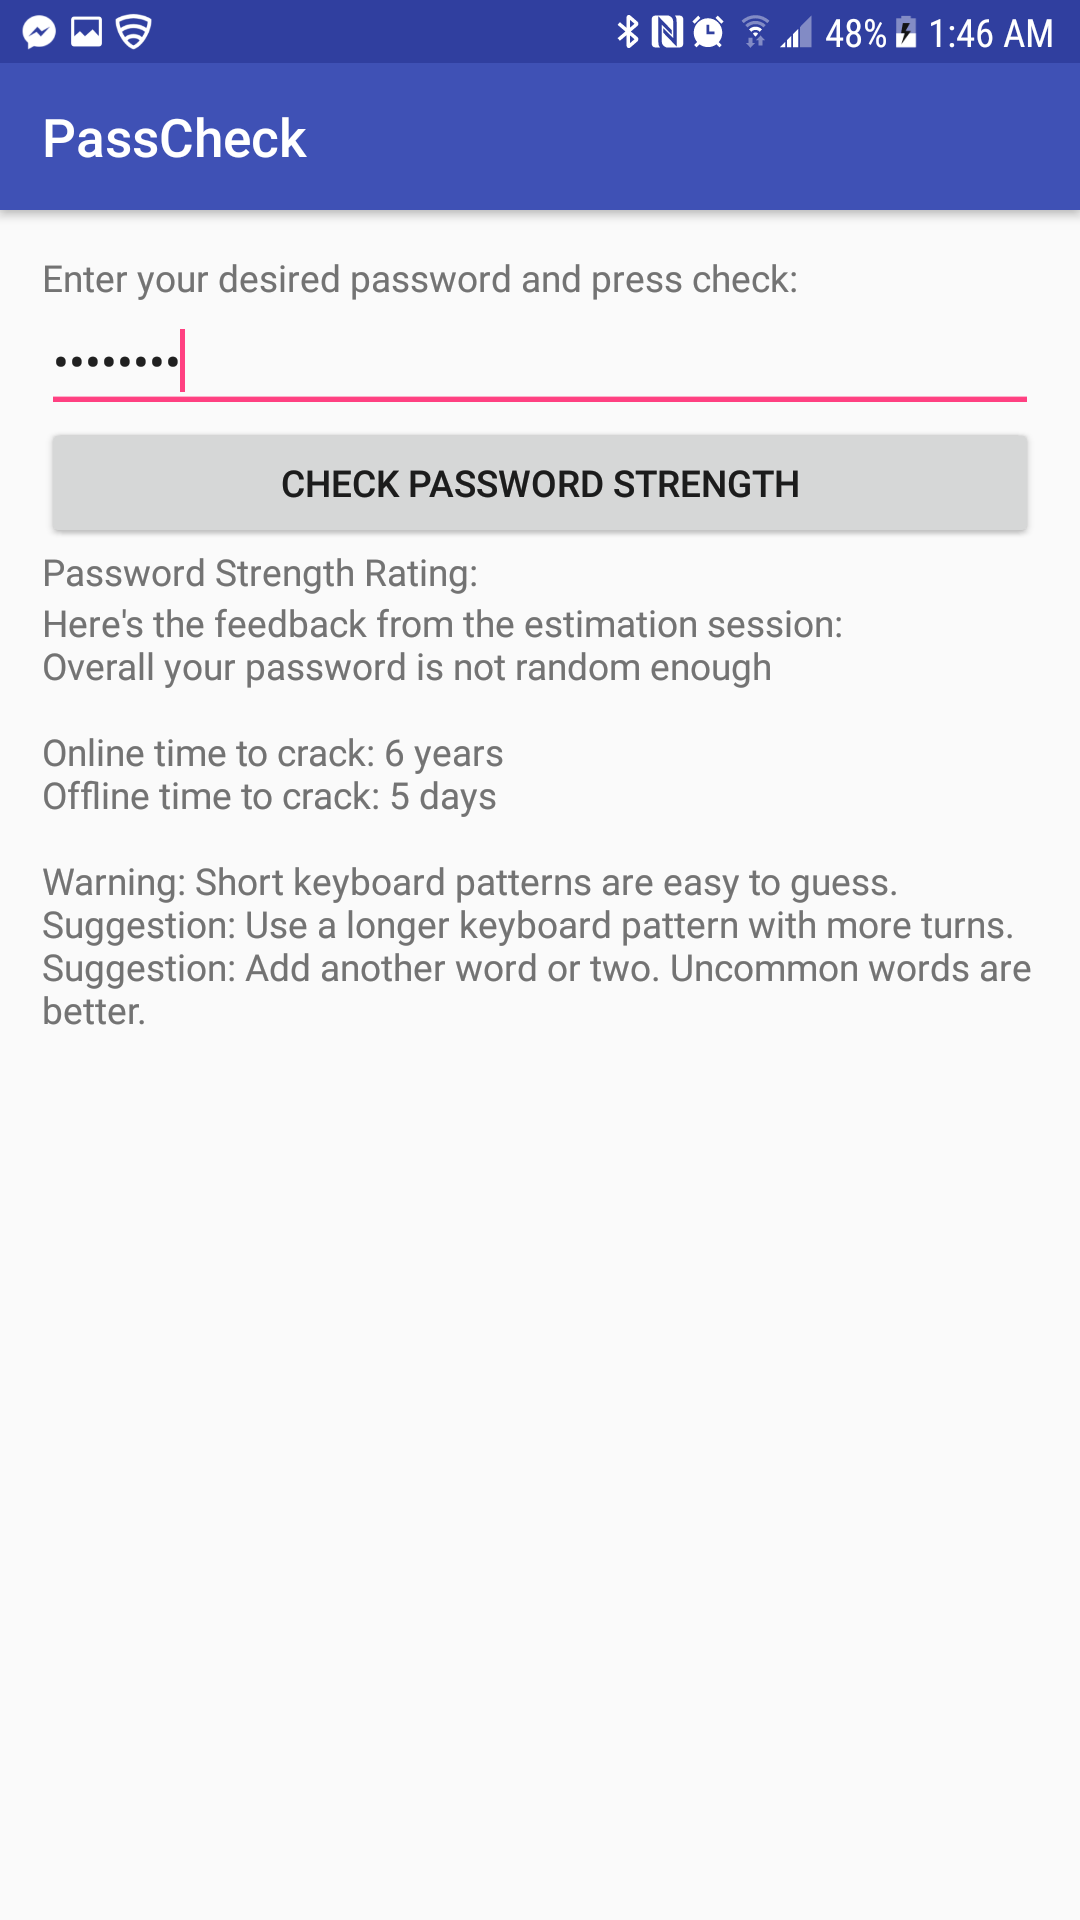
\includegraphics[width=3in]{img/t5s4.png}
        }
		\centering
		\caption{Task 5 - A few random symbols and letters}
	\end{figure}

	\begin{figure}[ht]
        \centerline{
            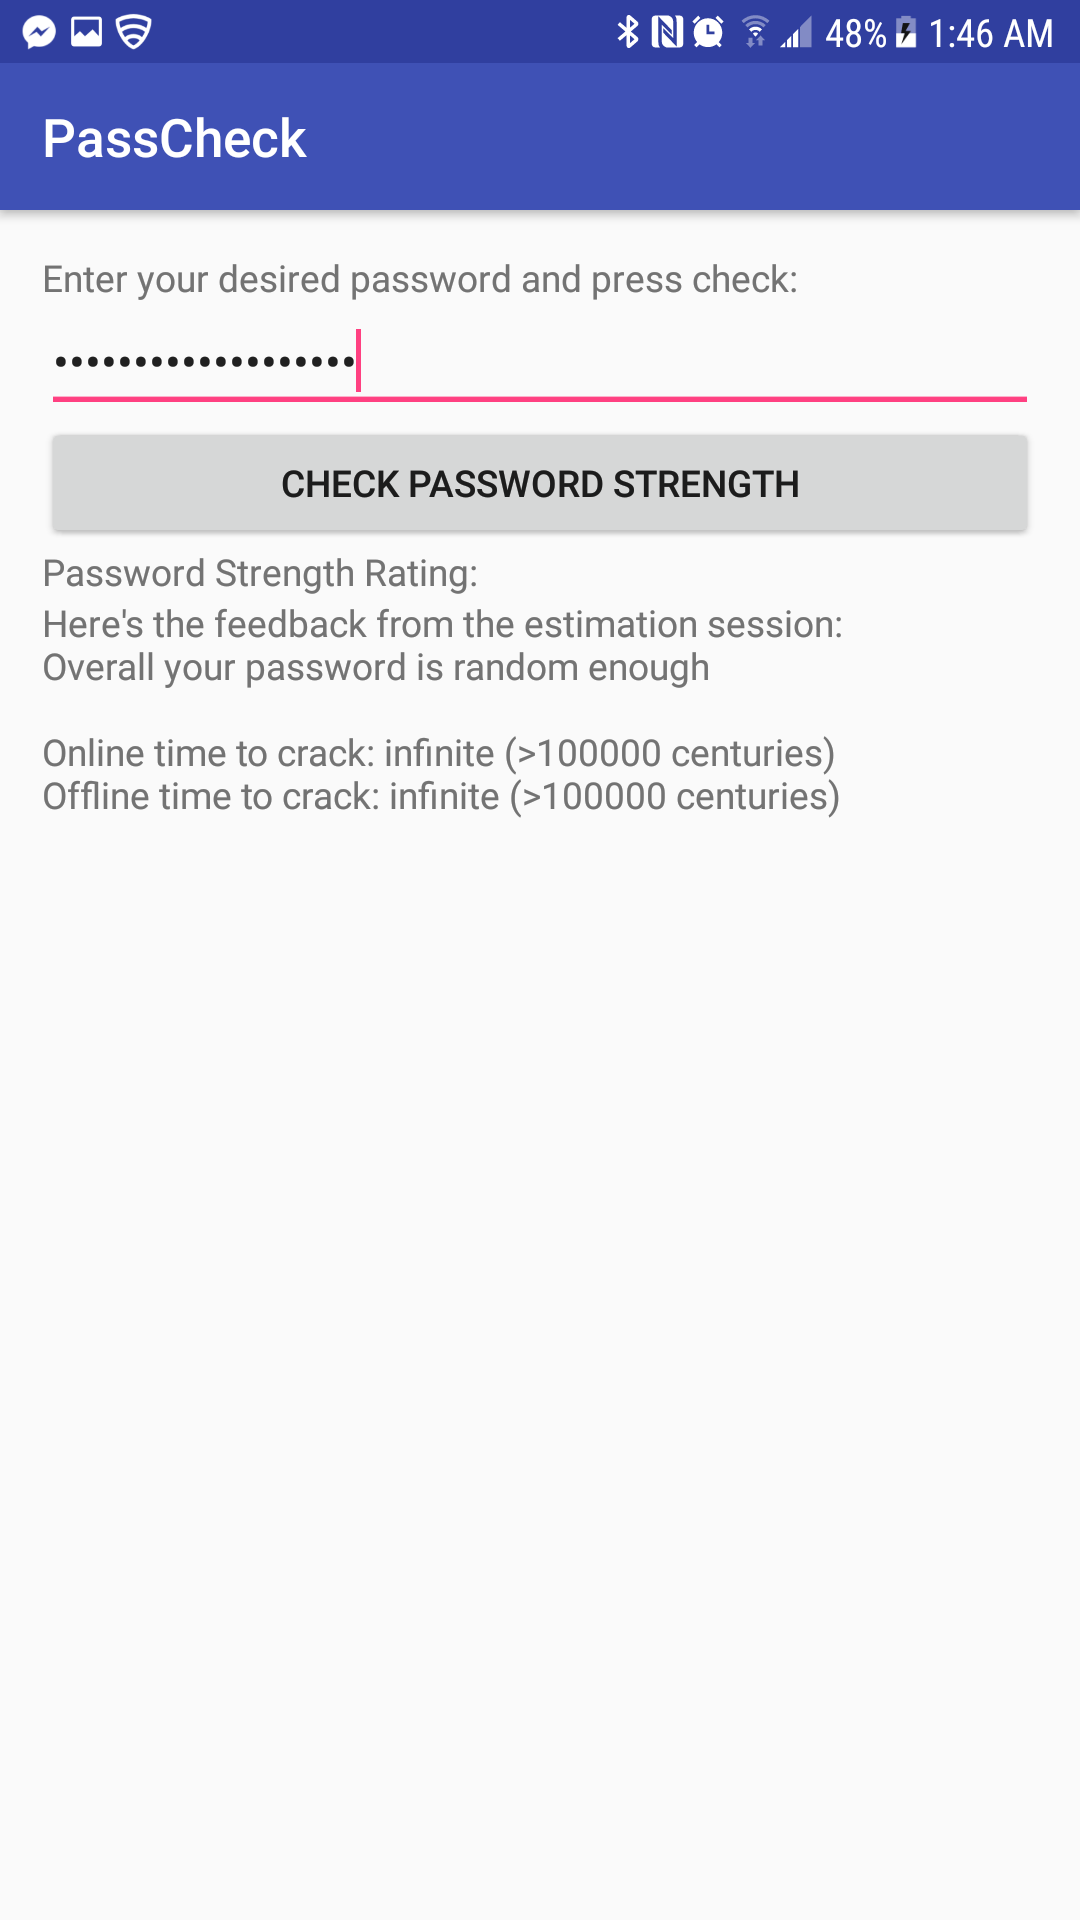
\includegraphics[width=3in]{img/t5s5.png}
        }
		\centering
		\caption{Task 5 - A bunch of random symbols, some random letters, and a word or two.}
	\end{figure}


\end{document}
